%%=================================================================
%% UFAC-modelo-TCC.tex (UTF-8 format), v1.0
%%
%%
%% Adaptação do Modelo de Trabalho de Conclusão de Curso (TCC) do
%% curso de Bacharelado em Sistemas de Informação da Universidade
%% Federal do Acre em LaTeX utilizando o pacote abnTeX2
%% (http://abnTeX2.googlecode.com).
%%
%% Precisa do arquivo abntex2-UFAC.sty e abntex2-alf.bst e
%% utilizando o compilador pdfLaTeX.
%%
%%
%% This work may be distributed and/or modified under the
%% conditions of the LaTeX Project Public License (LPPL), either
%% version 1.3 of this license or (at your option) any later
%% version.
%% The latest version of this license is in
%% http://www.latex-project.org/lppl.txt and version 1.3 or later
%% is part of all distributions of LaTeX version 2005/12/01 or
%% later.
%%
%% Further information about abnTeX2 are available on
%% https://www.abntex.net.br/
%%
%%
%% This work has the LPPL maintenance status `maintained'.
%%
%% The Creator and Current Maintainer of this work:
%% Manoel Limeira <juniorlimeiras@gmail.com>.
%%
%% Others contributors of this work:
%% Christopher Saar <cristophersaar@gmail.com>, Victor Alexandre<victoralexandre922@gmail.com>, Clécio Elias<https://github.com/Cleps>.
%%
%%
%% Última versão janeiro/2024
%%=================================================================

% MODIFIED: Adicionada opção chapter=TITLE para que os títulos dos capítulos, elementos pré-textuais e pós-textuais sejam escritos em maiúsculas
\documentclass[
    % -- opções da classe memoir --
    12pt,				       % Tamanho da fonte
    openright,			       % Capítulos começam em pág. ímpar (insere página vazia caso preciso)
    oneside,			       % Impressão apenas no anverso. Oposto a opção "twoside"
    a4paper,			       % Tamanho do papel
    % -- opções do pacote abntex2 --
    chapter=TITLE,             % Títulos de capítulos, de elementos pré-textuais e pós-textuais em maiúsculas
    sumario=tradicional,       % Sumário padrão memoir. Oposto a opção "abnt-6027-2012"
    % -- opções do pacote babel --
    english,			        % Idioma adicional para hifenização
    brazil, 				    % Idioma principal do documento
 ]{abntex2}


% ADDED: Importação do arquivo abntex2-alf.bst para que o sistema de citação seja (Autor, data) e dos pacotes datetime, xcolor, pgfplots, pgfplotstable e microtype para adicionar funcionalidades de arranjo visual do texto, plotagem de dados, estilização do texto, acesso de datas e horários
%% CONFIGURAÇÕES DE PACOTES

% Pacotes básicos
\usepackage{lmodern}			% Usa a fonte Latin Modern
\usepackage[T1]{fontenc}		% Seleção de códigos de fonte de saída
\usepackage[utf8]{inputenc}		% Codificação do documento (conversão automática dos acentos)
\usepackage{indentfirst}		% Indenta o primeiro parágrafo de cada seção
\usepackage{graphicx}			% Inclusão de gráficos e figuras
\usepackage{booktabs}           % \toprule, \midrule e \bottomrule para tabelas
\usepackage{datetime}           % Acesso de datas e horários na compilação

% MODIFIED: Adicionada opção abnt-etal-text=it para que "et al." seja escrito em itálico
% Sistema (Autor, data) com títulos das referências em negrito e termo latino "et al." escrito em itálico
\usepackage[alf,abnt-emphasize=bf, abnt-etal-text=it]{abntex2cite}
\bibliographystyle{abntex2-alf.bst}
% FUTURE-TODO: Modificar comando \cite para usar sistema (Autor, data) e não (AUTOR, data) sem precisar do arquivo .bst - apagar arquivo .bst e comando acima quando finalizado

% Títulos em fonte Times
\usepackage{mathptmx}
\renewcommand{\ABNTEXchapterfont}{\rmfamily\bfseries}

% Leitura de figuras .eps, compilação para PDF
\usepackage[outdir=./]{epstopdf}
\usepackage{epsfig}

\usepackage{abntex2-UFAC}       % Personalização de ESTILO para a Universidade Federal do Acre

% Pacotes adicionais

% Plotagem de dados
\usepackage{pgfplots, pgfplotstable} % mais detalhes veja https://pt.overleaf.com/learn/latex/Pgfplots_package
\pgfplotsset{compat=1.15} % resolve o problema do pacote pgfplots em múltiplas ferramentas de compilação

\usepackage{xcolor}             % Controle das cores

\usepackage{microtype} 			% Para aprimoramento do arranjo visual do texto na ferramenta OVERLEAF

% FUTURE-TODO: Modificar comandos relacionados as expressões latinas para serem escritas em itálico

% MODIFIED: Termos latinos para serem escritos em itálico
\renewcommand{\apudname}{\textit{apud}}
\renewcommand{\passimname}{\textit{passim}}
\renewcommand{\Idemname}{\textit{Id.}}
\renewcommand{\Ibidemname}{\textit{Ibid.}}
\renewcommand{\opcitname}{\textit{op.\ cit.}}
\renewcommand{\loccitname}{\textit{loc.\ cit.}}
\renewcommand{\cfcitename}{\textit{Cf.}}
\renewcommand{\etseqname}{\textit{et seq.}}
% ---

% MODIFIED: Textos para serem mais diversificados e datas para serem escritas de forma automática
%% Informações de dados para CAPA e FOLHA DE ROSTO
\titulo{Modelo para Trabalhos de Conclusão do Curso de Bacharelado em Sistemas de Informação da UFAC}

\autor{Nome Completo do (a) Autor (a)}

\local{Rio Branco}

\data{\the\year} % Automatiza a inserção do ano atual, para modificação por um ano específico troque "\the\year" pelo ano desejado

\orientador{Nome Completo do (a) Orientador (a)} % Redefinido no abntex2-UFAC.sty para aceitar Instituição (default = Curso de Bacharelado em Sistemas de Informação - Universidade Federal do Acre)

\coorientador{Nome Completo do (a) Coorientador (a)}

\instituicao{Universidade Federal do Acre}

% Campus ou Centro (opcional)
\campus{Centro de Ciências Exatas e Tecnológicas} % Pacote abntex2-UFAC

\curso{Curso de Bacharelado em Sistemas de Informação} % Pacote abntex2-UFAC

\membrobancaA[Curso de Bacharelado em Sistemas de Informação]{Membro (a) da Banca A} % Pacote abntex2-UFAC (default = Curso de Bacharelado em Sistemas de Informação - Universidade Federal do Acre)

\membrobancaB[Curso de Bacharelado em Sistemas de Informação - Instituto de Ensino de Algum Lugar]{Membro (a) da Banca B} % Pacote abntex2-UFAC (default = Curso de Bacharelado em Sistemas de Informação - Universidade Federal do Acre)

\databanca{\today} % Automatiza a inserção da data atual, para modificação por uma data específica troque "\today" pela data desejada por extenso

% REMOVED: Comando \preambulo por ter sido inutilizado no abntex2-UFAC.sty
% O preambulo deve conter o tipo do trabalho (tese, dissertação, trabalho de conclusão de curso e outros); objetivo (aprovação em disciplina, grau pretendido e outros); nome da instituição a que é submetido e a área de concentração
% \preambulo{Monografia apresentada como Trabalho de Conclusão de Curso, exigência para obtenção do grau de Bacharel em Sistemas de Informação, na Universidade Federal do Acre}
% ---

%% Configurações de aparência do PDF final

% informações para o arquivo pdf de saída
\makeatletter

% MODIFIED: Cores de links do documento
\hypersetup{
    % metadados
    pdftitle={\@title},
    pdfauthor={\@author},
    pdfsubject={\imprimirpreambulo},
    pdfcreator={LaTeX with abnTeX2},
    %%% IMPORTANTE: ALTERAR "colorlinks=false" PARA "colorlinks=true" ANTES DE IMPRIMIR A VERSÃO FINAL DO DOCUMENTO
    colorlinks=false,           % false: links em frame; true: links coloridos
    linkcolor=black,            % cor dos links no documento
    citecolor=black,            % cor dos links para a bibliografia
    filecolor=black,            % cor dos links para arquivos
    urlcolor=black,             % cor dos links para sites
    bookmarksdepth=4,           % profundidade do sumário do PDF
}

\makeatother
% ---

\begin{document}
% Retira espaço extra obsoleto entre as frases
\frenchspacing


% ----------------------------------------------------------
% ELEMENTOS PRÉ-TEXTUAIS
% ----------------------------------------------------------
\pretextual


%% Capa
\imprimircapa
% ---

%% Folha de rosto
\imprimirfolhaderosto
% ---

%% Folha de aprovação
\imprimirfolhadeaprovacao
% ---

% MODIFIED: Comandos para dedicatória ser impressa no local correto
%% Dedicatória (opcional)
% Dedicatória(s): Elemento opcional, texto em que o autor presta homenagem ou dedica seu trabalho \cite{NBR14724:2011}
\begin{dedicatoria}
    \vspace*{\fill}

    \begin{flushright}
        \begin{minipage}{0.5\textwidth} % minpage + 0.5\textwidth para ocupar metade da largura da página
            \raggedleft{Obrigado pela atualização de modelo ABNT, Christopher e Victor.}
        \end{minipage}
    \end{flushright}

    \vspace*{2cm}
\end{dedicatoria}
% ---

%% Agradecimentos (opcional)
\begin{agradecimentos}
    % inserir o texto de agradecimentos aqui
    Elemento opcional, texto colocado ap\'os a dedicat\'oria em que o autor faz agradecimentos dirigidos àqueles que contribuíram de maneira relevante à elaboração do trabalho~\cite{NBR14724:2011}.
\end{agradecimentos}
% ---

% MODIFIED: Comandos para epígrafe ser impressa no local correto e texto
%% Epígrafe
\begin{epigrafe}
    \vspace*{\fill}

    \begin{flushright}
        \begin{minipage}{0.5\textwidth} % minpage + 0.5\textwidth para ocupar metade da largura da página
            % REMOVED: Itálico desnecessário no texto da epígrafe
            % \raggedleft{\textit{``Word? nunca mais.''\\ (Qualquer usuário de \LaTeX)}}
            \raggedleft{``Word? nunca mais.'' \\ (Algum usuário de \LaTeX)}
        \end{minipage}
    \end{flushright}

    \vspace*{2cm}
\end{epigrafe}
% ---

% MODIFIED: Texto e comando de citação
%% Resumo em português
\begin{resumo}
    \noindent
    % inserir o resumo aqui
    Segundo~\citeonline{NBR6028:2003}, o resumo é elemento obrigat\'orio, constitu\'ido de uma sequ\^encia de frases concisas e objetivas e n\~ao de uma simples enumera\c c\~ao de t\'opicos, não ultrapassando 500 palavras. Além disso, o resumo deve ressaltar o objetivo, o método, os resultados e as conclusões do documento. A ordem e a extensão destes itens dependem do tipo de resumo (informativo ou indicativo) e do tratamento que cada item recebe no documento original.
    \vspace{\onelineskip}

    \noindent
    \textbf{Palavras-chave}: Palavras representativas do conteúdo do trabalho, isto é, palavras-chave e/ou descritores, conforme a ABNT NBR 6028~\cite{NBR6028:2003}.
\end{resumo}
%% ---

% MODIFIED: Texto
%% Resumo em inglês
\begin{resumo}[Abstract]
    \begin{otherlanguage*}{english}
        \noindent
        % inserir o abstract aqui
        According to~\cite{NBR6028:2003}, the abstract is a mandatory element, consisting of a sequence of concise and objective sentences, not just a simple enumeration of topics, and should not exceed 500 words. Additionally, the abstract should highlight the objective, method, results, and conclusions of the document. The order and extent of these items depend on the type of abstract (informative or indicative) and how each item is treated in the original document.
        \vspace{\onelineskip}

        \noindent
        \textbf{Key-words}: Representative words of the content of the work, that is, keywords and/or descriptors, according to ABNT NBR 6028~\cite{NBR6028:2003}.
    \end{otherlanguage*}
\end{resumo}
%% ---

%% Lista de ilustrações
\pdfbookmark[0]{\listfigurename}{lof}
\listoffigures*
\cleardoublepage
% ---

% ADDED: Comando para imprimir lista de quadros
%% Lista de quadros
\pdfbookmark[0]{\listofquadrosname}{loq}
\listofquadros*
\cleardoublepage
% ---

%% Lista de tabelas
\pdfbookmark[0]{\listtablename}{lot}
\listoftables*
\cleardoublepage
% ---

% MODIFIED: Texto
%% Lista de siglas e abreviaturas (opcional)
% sintaxe: \item [sigla] Descrição da sigla
\begin{siglas}
	\item[ABNT] Associação Brasileira de Normas Técnicas
	\item[UFAC] Universidade Federal do Acre
\end{siglas}
%% ---

% MODIFIED: Exemplos de símbolos
%% Lista de símbolos (opcional)
% sintaxe: \item [simbolo] Descrição do símbolo
\begin{simbolos}
    \item[$\infty$] Infinito
    \item[$\Gamma$] Letra grega Gama
    \item[$\Lambda$] Lambda
    \item[$\zeta$] Letra grega minúscula zeta
    \item[$\in$] Pertence
\end{simbolos}
%% ---

%% Sumário
\pdfbookmark[0]{\contentsname}{toc}
\tableofcontents*
\cleardoublepage
% ---


% ----------------------------------------------------------
% ELEMENTOS TEXTUAIS
% ----------------------------------------------------------
\textual


% MODIFIED: Adição de quebras de linha para início de parágrafos corretamente, troca de links quebrados, adição ou ajuste de textos de exemplo, posição da legenda e adição de fonte nas figuras e tabelas nos elementos textuais

% ADDED: Comando \pagestyle{simple} para remoção do cabeçalho no modelo Capítulo <N>. <Nome do Capítulo>
\pagestyle{simple}

% Modifique a estrutura dos capítulos e seções de acordo com a necessidade do seu trabalho

%% Introdução
\chapter{Introdução}\label{sec:introducao}
% inserir o texto abaixo
Apresentar uma visão geral do assunto que será abordado no trabalho, procurando fazer com que o leitor adquira uma compreensão inicial do que será tratado e fornecendo informações que o levem a perceber a sua importância.

% FUTURE-TODO: Fazer comando \ref e \autoref reconhecerem o número dos elementos como tabelas, figuras, quadros e outros corretamente
Abaixo na Figura 1 temos um exemplo de Figura.

\begin{figure}[!ht]
    \centering
    \textbf{\caption{Exemplo de figura.}}
    \includegraphics[width=0.3\linewidth]{figuras/exefig.eps}
    \label{fig:exefig}
    \fonte{\cite{site2019}}
\end{figure}

Escrever bem é uma arte que exige muita técnica e dedicação. Há vários bons livros sobre como escrever uma boa dissertação ou tese. Para a escrita de textos em Ciência da Computação, Writing for Computer Science~\cite{zobel2014} é uma leitura obrigatória. O livro Metodologia de Pesquisa para Ciência da Computação~\cite{wazlawick2009} também merece uma boa lida.

Alguns links interessantes para se trabalhar com a classe abn\TeX\ e \LaTeX\ em geral\footnote{E também para usar alguns comandos de citação como exemplo}:

\begin{alineas}
    \item Informações da classe Abn\TeX: \citeonline{abntex2classe}
    \item Ajustes nas citações e referências: \citeonline{abntex2cite} e \citeonline{abntex2cite-alf}
    \item Classe memoir (base do Abn\TeX\ ): \apudonline{memoir}{abntex2classe}
    \item Livros interessantes sobre \LaTeX: \cite{Dongen2012,LeslieLamport90,FrankMittelbach111,Dongen2012}
    \item Distribuição \LaTeX\ com múltiplas ferramentas: \url{http://miktex.org/}
    \item Editor \LaTeX\ gratuito: \url{http://texstudio.sourceforge.net/}
    \item Editor \LaTeX\ \textit{online} gratuito: \url{https://www.overleaf.com}
    \item Gerenciador de arquivos \texttt{.bib}: \url{http://jabref.sourceforge.net/}
    \item Gerenciador de artigos: \url{http://www.mendeley.com/}
    \item Exemplo de Tabela IBGE na Tabela 2 no \autoref{sec:cronograma}
    \item Exemplo de Quadro no Capítulo \ref{sec:metodos}
\end{alineas}

\section{Problema da Pesquisa}\label{sec:ProbPesq}
% inserir o texto abaixo
Qual a grande questão que se busca responder? Qual o problema se presente resolver? \\
O problema é a mola propulsora de todo o trabalho de pesquisa. Após definido o tema, levanta-se uma questão para ser respondida através de uma hipótese, que será confirmada ou negada através do trabalho de pesquisa. O problema é criado pelo próprio autor e relacionado ao tema escolhido. O autor, no caso, criará um questionamento para definir a abrangência de sua pesquisa. Não há regras para se criar um problema, mas alguns autores sugerem que ele seja expresso em forma de pergunta.
De 1 a 2 páginas

\section{Objetivos}\label{sec:objetivos}
% inserir o texto abaixo
O objetivo da pesquisa deve ser diretamente verificável ao final do trabalho. Um bom objetivo de pesquisa possivelmente irá demonstrar que alguma hipótese sendo testada é ou não verdadeira.

% MODIFIED: Níveis de seções de objetivos gerais e específicos - caso específico de TCC II do curso de Sistemas de Informação

\subsection{Objetivo Geral}\label{sec:ObjGeral}
% inserir o texto abaixo
Qual o objetivo maior do trabalho?

\subsection{Objetivos Específicos}\label{sec:ObjEspec}
% inserir o texto abaixo
Os objetivos específicos do trabalho devem ser expressos na forma de uma condição não trivial cujo sucesso possa vir a ser verificado ao final do trabalho. Um objetivo bem expresso em geral terá verbos como “demonstrar”, “provar”, “melhorar” (de acordo com alguma métrica definida), etc.

Deve-se tomar cuidado com certos verbos que determinam objetivos cuja verificação é trivial e, portanto, inadequada. Entre eles pode-se citar “propor”, “estudar”, “apresentar”, etc. Se o objetivo do trabalho é propor algo, basta que a coisa seja proposta para que o objetivo seja atingido e, portanto, essa forma é trivial e inadequada, pois a definição do objetivo não menciona a qualidade daquilo que será proposto.

Se o objetivo do trabalho é estudar algo, então ele terá sido alcançado se aquilo foi estudado, não importando se alguma nova informação foi aprendida ou não, sendo, portanto, inadequado como objetivo de pesquisa. Estudar, normalmente, é o objetivo do aluno e não do trabalho.

Se o objetivo do trabalho consiste em apresentar algo, novamente ele é trivial e inadequado. Uma simples apresentação não produz necessariamente conhecimento novo. Por exemplo, “o objetivo deste trabalho é apresentar os operadores da lógica booleana”; tal objetivo pode ser alcançado com um pequeno texto explicando os operadores conhecidos, mas, como não traz informação nova, não é um objetivo de pesquisa.

Insira os objetivos específicos no formato de tópicos.

\section{Justificativa da Pesquisa}\label{sec:Justificativa}
% inserir o texto abaixo
A proposta, o estudo e a apresentação podem ser justificáveis como objetivo de pesquisa desde que o objeto da proposta, estudo ou da apresentação seja algo original~\cite{wazlawick2009}.

A Justificativa num projeto de pesquisa, como o próprio nome indica, é o convencimento de que o trabalho de pesquisa é fundamental de ser efetivado. O tema escolhido pelo pesquisador e a Hipótese levantada são de suma importância, para a sociedade ou para alguns indivíduos, de ser comprovada.

Deve-se tomar o cuidado, na elaboração da Justificativa, de não se tentar justificar a hipótese levantada, ou seja, tentar responder ou concluir o que vai ser buscado no trabalho de pesquisa. A Justificativa exalta a importância do tema a ser estudado, ou justifica a necessidade imperiosa de se levar a efeito tal empreendimento.
Por que será feita a pesquisa sobre este assunto? Aqui a importância do tema. Qual a importância em se pesquisar este assunto?


\section{Metodologia}\label{sec:Metodologia}
% inserir o texto abaixo
Como será realizado a monografia? Pesquisa bibliográfica, estudo de caso, levantamento (ver manual sobre metodologia no grupo) \\
Detalhar se tem instrumentos de coleta de dados (questionário, formulário, entrevista, observação), quem é a população e a amostra. Como serão tabulados os dados.

A Metodologia é a explicação minuciosa, detalhada, rigorosa e exata de toda ação desenvolvida no método (caminho) do trabalho de pesquisa.

É a explicação do tipo de pesquisa, do instrumental utilizado (questionário, entrevista etc), do tempo previsto, da equipe de pesquisadores e da divisão do trabalho, das formas de tabulação e tratamento dos dados, enfim, de tudo aquilo que se utilizou no trabalho de pesquisa.

Se for desenvolvimento de sistemas ou de aplicações falar quais ferramentas serão utilizadas.


\section{Organização}\label{sec:Organizacao}
% inserir o texto abaixo
O que tem em cada um dos capítulos seguintes (Detalhar a estrutura de capítulos que será adotada, partindo desde o 1º capítulo da monografia até as referências).
%% ---

%% Referencial teórico ou Fundamentação teórica
\chapter{Referencial Teórico}\label{sec:RefTeorico}
% Insirir texto abaixo
Parte teórica a monografia: qual o assunto que dá o embasamento para a monografia? Quais os principais temas que precisam ser abordados? Dividir os temas em subtítulos.

As referências dos documentos consultados para a elaboração do Projeto é um item obrigatório. Nela constam normalmente os documentos e qualquer fonte de informações consultadas no Levantamento de Literatura.

Podem ser feitos diversos capítulos diferentes para a fundamentação teórica, conforme a necessidade.

Geralmente de 3 a 5 páginas baseadas em autores (de preferência livros) usando as normas metodológicas para citá-los. Referências de Internet devem ser realizadas com cuidado, não exceder a 30\% das obras citadas. \\

\textbf{Exemplo de referências:}

Em caso de citar, um metadado específico definido no .bib, como o nome do autor \verb|\authoronline{...}| e o ano de publicação do trabalho \verb|citeyear{...}| como em:
(\citeauthoronline{NBR14724:2011}, \citeyear{NBR14724:2011}).

E em caso de citação tradicional, utilizando o \verb|\cite{...}| como em:
\cite{NBR14724:2011}.

Exemplo de Tabela: ver Tabela 1.

\begin{table}[!ht]
    \begin{center}
        \textbf{\caption{Distribuição IMC em Adultos}}
        \label{tab:exetab}
        \begin{tabular}{| c | c |}
            \hline
            \textbf{Classificação} & \textbf{IMC} \\
            \hline\hline
            Baixo Peso & < 18,5 \\
            Peso Adequado & > 18,5 e < 25 \\
            Sobrepeso & > 25 e < 30 \\
            Obesidade & > 30 \\
            \hline
        \end{tabular}
    \end{center}
    \fonte{Elaboração Própria}
\end{table}

Na Figura 2 temos um exemplo de figura com uma figura de exemplo de citação.

\begin{figure}[!ht]
    \centering
    \textbf{\caption{Exemplo de figura com exemplo de citação.}}
    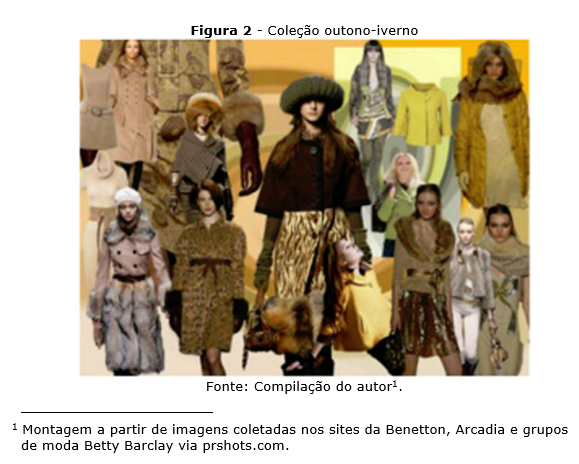
\includegraphics[width=0.95\linewidth]{figuras/execite.png}
    \label{fig:execite}
    \fonte{\cite{gogoni_refimage_2021}}
\end{figure}

Não termine um capítulo ou seção com uma figura ou tabela. Insira um texto após a figura ou tabela de preferência um texto ligando a seção atual com a próxima.
%% ---

%% Capítulo ou seção de trabalhos relacionados (opcional)
\section{Trabalhos Relacionados}\label{sec:TrabRel}
% \chapter{Trabalhos Relacionados}\label{sec:TrabRel}
% inserir o texto abaixo

%% ---

%% Capítulo de desenvolvimento, materiais e métodos ou estudo de caso (nome a escolha do aluno)
\chapter{Materiais e Métodos}\label{sec:metodos}
% inserir o texto abaixo

% ADDED: Exemplo de quadro implementado
Exemplo de Quadro (dados qualitativos): ver o Quadro 1.

\begin{quadro}[!ht]
    \centering
    \textbf{\caption{Comparativo de trabalhos relacionados}}
    \begin{tabular}{|p{2.1cm}|l|p{4.1cm}|p{2.1cm}|p{3.1cm}|} \hline
        % Títulos
        \textbf{Trabalho}
        & \textbf{SGBD}
        & \textbf{Objetivo}
        & \textbf{Abordagem}
        & \textbf{Avaliação de custo}
        \\ \hline
        % Coluna 1
        \cite{Alagiannis:2010}
        & PostgreSQL
        & Sugestão de índices e particionamento
        & \emph{Offline} e \emph{online}
        & Uso de componente \emph{what-if}, acessando otimizador do SGBD para avaliar custo da consulta com \emph{cache} dos resultados
        \\ \hline
        % Coluna 2
        \cite{Agrawal:2004}
        & SQL Server
        & Sugestão de índices, particionamento e materialização de dados
        & \emph{Offline}
        & Uso de componente \emph{what-if}, acessando otimizador do SGBD para avaliar custo da consulta
        \\ \hline
        % Coluna 3
        \cite{Zilio:2004}
        & DB2
        & Sugestão de índices, particionamento, materialização de dados e agrupamento multidimensional
        & \emph{Offline}
        & Uso de componente \emph{what-if}, acessando otimizador do SGBD para avaliar custo da consulta
        \\ \hline
    \end{tabular}
    \label{qua:exequa}
    \fonte{Adaptado de~\cite{weiland_latex-unisc_2022}}
\end{quadro}

Não termine um capítulo ou seção com uma figura ou tabela. Insira um texto após a figura ou tabela de preferência um texto ligando a seção atual com a próxima.
%% ---

%% Capítulo de Resultados
\chapter{Resultados}\label{sec:resultados}
% inserir o texto abaixo

% ---

%% Cronograma
\chapter{Cronograma}\label{sec:cronograma}
% inserir o texto abaixo
Sempre insira texto entre as tabelas e figuras para que as mesmas não fiquem soltas na dissertação.

\begin{table}[htbp]
    \centering
    \textbf{\caption[Cronograma Normal]{Cronograma do Projeto em Meses}}
    \label{tab:cronograma1}
    \begin{tabular}{lcccccccccccc} %|c|c|c|c|c|c|c|c|c|c|c|c
        \toprule
        \textbf{Atividade} & \textbf{1} & \textbf{2} & \textbf{3} & \textbf{4} & \textbf{5} & \textbf{6} & \textbf{7} & \textbf{8} & \textbf{9} & \textbf{10} & \textbf{11} & \textbf{12} \\
        \midrule
            Revisão Bibliográfica & $\bullet$ & $\bullet$ & & & & & & & & & & \\
            Métodos & & & $\bullet$ & $\bullet$ & & & & & & & & \\
            Testes & & & & $\bullet$ & $\bullet$ & $\bullet$ & & & & & & \\
            Resultados & & & & & & & $\bullet$ & $\bullet$ & & & & \\
            Conclusão & & & & & & & $\bullet$ & $\bullet$ & $\bullet$ & & & \\
            Banca & & & & & & &&&& $\bullet$ & $\bullet$ & $\bullet$ \\
        \bottomrule
    \end{tabular}
    \fonte{Elaboração própria}
\end{table}

O abn\TeX\ introduziu o comando \texttt{IBGEtab} para formatação de tabelas. Um exemplo de tabela convencional do \LaTeX\ pode ser observado na Tabela 2 enquanto um exemplo usando o \texttt{IBGEtab} é mostrado na Tabela 3.

\begin{table}[htbp]
    \IBGEtab{
        \textbf{\caption[Cronograma (IBGE)]{Cronograma do Projeto em Meses usando o comando IBGEtab para a formatação da tabela}}
        \label{tab:cronogramaIBGE}
    }{
    \begin{tabular}{lcccccccccccc} %|c|c|c|c|c|c|c|c|c|c|c|c
        \toprule
        \textbf{Atividade} & \textbf{1} & \textbf{2} & \textbf{3} & \textbf{4} & \textbf{5} & \textbf{6} & \textbf{7} & \textbf{8} & \textbf{9} & \textbf{10} & \textbf{11} & \textbf{12} \\
        \midrule
            Revisão Bibliográfica & $\bullet$ & $\bullet$ & & & & & & & & & & \\
            Métodos & & & $\bullet$ & $\bullet$ & & & & & & & & \\
            Testes & & & & $\bullet$ & $\bullet$ & $\bullet$ & & & & & & \\
            Resultados & & & & & & & $\bullet$ & $\bullet$ & & & & \\
            Conclusão & & & & & & & $\bullet$ & $\bullet$ & $\bullet$ & & & \\
            Banca & & & & & & &&&& $\bullet$ & $\bullet$ & $\bullet$ \\
        \bottomrule
    \end{tabular}%
    }\centering{
    \fonte{Fonte: Elaboração própria}}
\end{table}%

Sempre cite as tabelas e figuras quando for usá-las na dissertação para gerar concordância de uso e apresentação dos elementos no texto e não faça a primeira citação da tabela ou figura longe de onde as mesmas foram posicionadas.

\begin{table}[!ht]
    \begin{center}
        \textbf{\caption{Cronograma do Projeto em Meses Alternativo.}}
        \label{tab:cronograma2}
        \begin{tabular}{lcccccccccccc} %|c|c|c|c|c|c|c|c|c|c|c|c
            \toprule
            \textbf{Atividade} & \textbf{1} & \textbf{2} & \textbf{3} & \textbf{4} & \textbf{5} & \textbf{6} & \textbf{7} & \textbf{8} & \textbf{9} & \textbf{10} & \textbf{11} & \textbf{12} \\
            \midrule
                Revisão Bibliográfica & $\bullet$ & $\bullet$ & & & & & & & & & & \\
                Métodos & & & $\bullet$ & $\bullet$ & & & & & & & & \\
                Testes & & & & $\bullet$ & $\bullet$ & $\bullet$ & & & & & & \\
                Resultados & & & & & & & $\bullet$ & $\bullet$ & & & & \\
                Conclusão & & & & & & & $\bullet$ & $\bullet$ & $\bullet$ & & & \\
                Banca & & & & & & &&&& $\bullet$ & $\bullet$ & $\bullet$ \\
            \bottomrule
        \end{tabular}%
        \fonte{Elaboração própria.}
    \end{center}
\end{table}

Não termine um capítulo ou seção com uma figura ou tabela. Insira um texto após a figura ou tabela de preferência um texto ligando a seção atual com a próxima.
%% ---


% ----------------------------------------------------------
% ELEMENTOS PÓS-TEXTUAIS
% ----------------------------------------------------------
\postextual


%% Referências bibliográficas
\bibliography{referencias.bib}\thispagestyle{empty}
%% ---

% Caso seja necessário glossário em seu documento, fazer a mão ou consulte o manual do pacote abnTeX2 para orientações sobre glossários prontos.

% FUTURE-TODO: implementar modelo simples de glossário
%% Glossário (opcional)
% \begin{glossario}
%     \item[LaTeX] Ferramenta de computador para autoria de documentos criada por D. E. Knuth
%     \item[abnTeX2] Suíte para LaTeX que atende os requisitos das normas da ABNT para elaboração de documentos técnicos e científicos brasileiros
% \end{glossario}
%% ---

% Caso sejam necessários apêndices ou anexos em seu documento use os ambientes abaixo

%% Apêndices
\begin{apendicesenv} \thispagestyle{empty}
    \partapendices % Imprime uma página indicando o início dos apêndices

    \chapter{Primeiro Apêndice} \thispagestyle{empty}
    % inserir seu apêndice abaixo

    \chapter{Segundo Apêndice} \thispagestyle{empty}
    % inserir seu apêndice abaixo
\end{apendicesenv}
%% ---

%% Anexos
\begin{anexosenv}
    \partanexos % Imprime uma página indicando o início dos anexos

    \chapter{Primeiro Anexo} \thispagestyle{empty}
    % inserir seu anexo abaixo

    \chapter{Segundo Anexo} \thispagestyle{empty}
    % inserir seu anexo abaixo
\end{anexosenv}
%% ---


\end{document}
